\chapter{Gait generation via IS-MPC}
\label{ch:ISMPC}
In the last chapter, we have given an overview on humanoid locomotion dynamics,
focusing in particular on the model of the Linear Inverted Pendulum (LIP). We have
described its dynamics, we have seen that it is unstable, and we have given a
condition for contact equilibrium on non-coplanar surfaces for the humanoid.
In this chapter, we exploit the previously
presented analysis to develop a gait generation scheme for humanoid locomotion
in a \textit{world of stairs}, an uneven terrain where all contact surfaces 
are piecewise horizontal.

The approach adopted in this manuscript is based on
Intrinsically-Stable MPC (IS-MPC) \cite{Scianca2020TRO},
a model predictive control scheme which, given as input a \textit{footstep plan}
(which defines the desired motion of the robot at high-level specifying desired
footstep positions, orientations, single and double support durations, and swing
foot trajectories), generates
a stable center of mass (CoM) trajectory, which can be tracked by a whole-body
controller. In IS-MPC, where the model is the one of the LIP, stability is
guaranteed via a stability constraint, which
bounds the displacement between the CoM and the zero-tilting moment point (ZMP).
Moreover, dynamic balance is enforced via constraints on the ZMP
position. In particular, since the polyhedral cone of eq.
\eqref{eq:ZMP-polyhedral-cone} would result in a nonlinear constraint, it is
conservatively approximated with a convex region. Because both constraints are 
linear, IS-MPC can be formulated as a Quadratic Programming (QP) program, and 
solved efficiently at each control iteration.

This chapter presents IS-MPC in its entirety, describing the prediction model (a LIP with a 
dynamic extension on the ZMP), the \textit{stability constraint} and the \textit{ZMP constraint}, and the
definition of the QP problem. In the end, the condition of feasibility of IS-MPC
optimization problem is discussed.

\section{Preliminaries}
TODO: basic behavior of IS-MPC with block scheme.
\begin{figure}
    \centering
    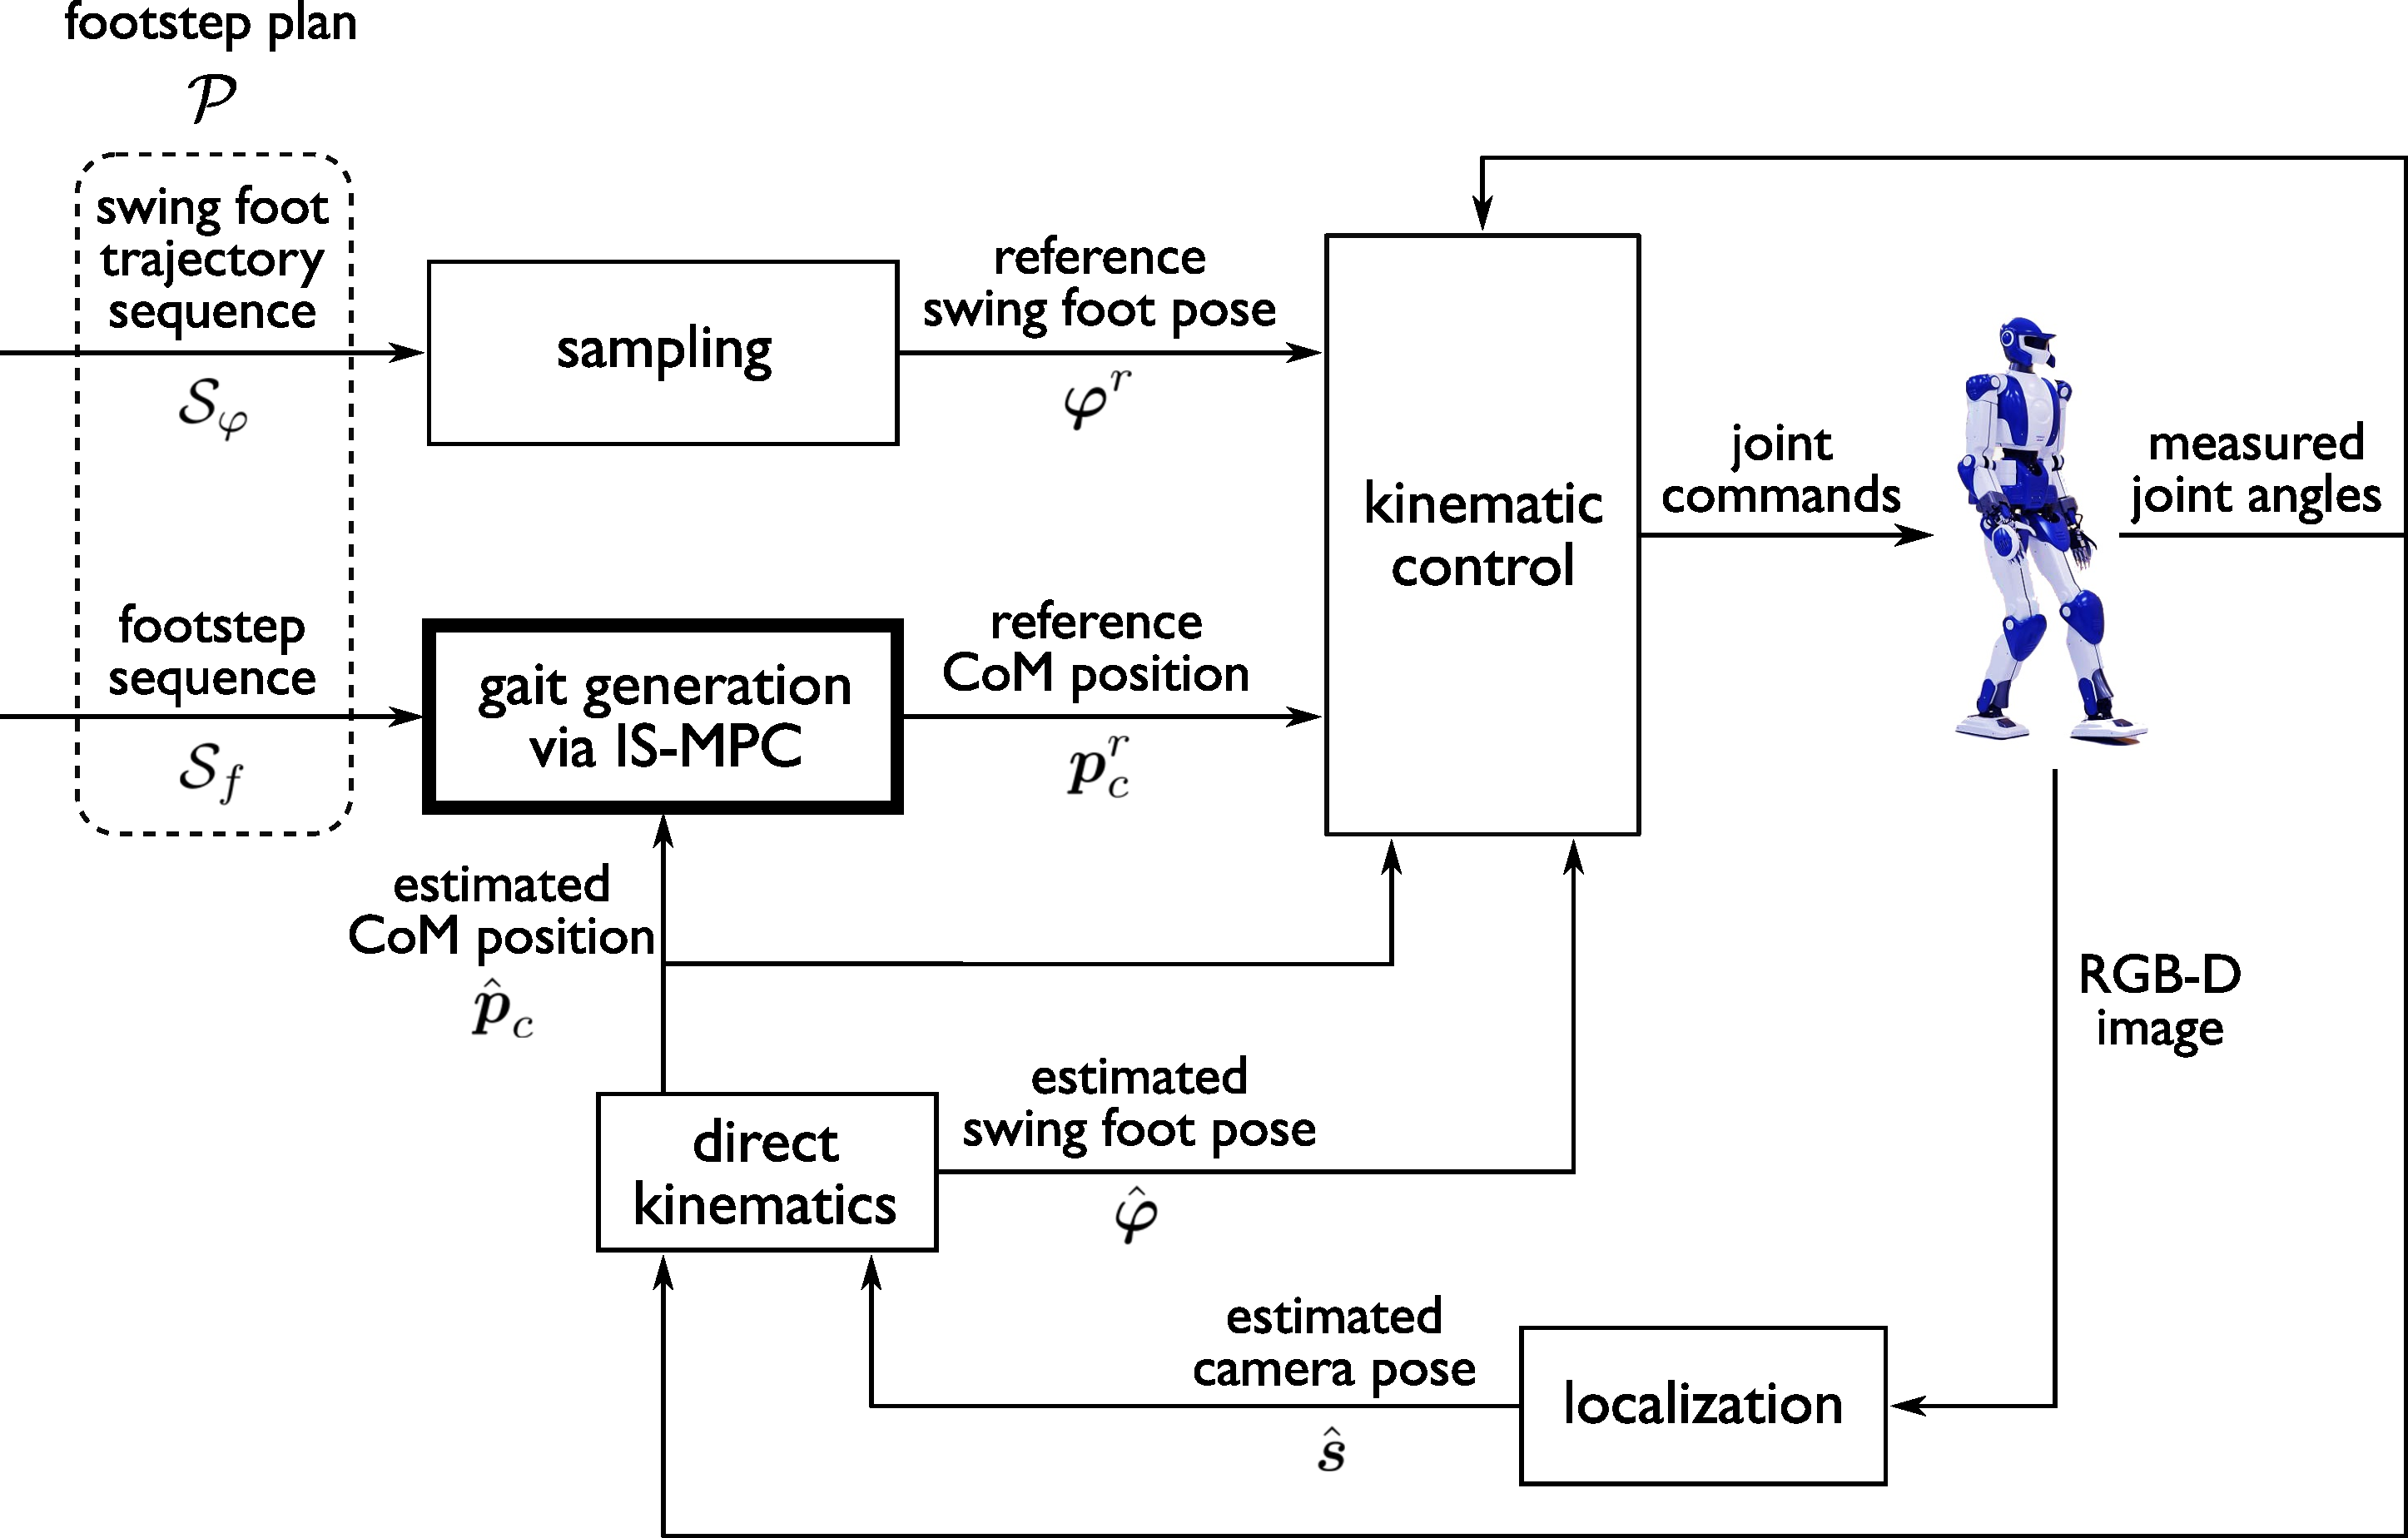
\includegraphics[width=\textwidth]{figures/BlockSchemeISMPC.pdf}
    \caption{Block scheme of IS-MPC.}
\end{figure}

\subsection{Footstep plan}
Definition of input of IS-MPC.

\section{Prediction model}
As already mentioned in Sec. \ref{sec:DynamicsHumanoidLocomotion:LinearInvertedPendulum},
control of the ZMP can be achieved by using the LIP model, which relates the 
position of the ZMP and the acceleration of the CoM. In order to obtain smoother
trajectories, we dynamically extend the LIP model \eqref{eq:LIPM}, obtaining a
model with derivative of the ZMP $\dot{\bm{p}}_z$ as control input. Denoting
the CoM as $\bm{p}_c = (x_c \; y_c \; z_c)^T$ and the ZMP as $\bm{p}_z = (x_z \; y_z \; z_z)^T$, the 
model can hence be rewritten as
\begin{equation*}
    \label{eq:LIPM-x-dynamic-extension}
    \begin{bmatrix}
        \dot{x}_c \\ \ddot{x}_c \\ \dot{x}_z 
    \end{bmatrix}
    =
    \begin{bmatrix}
        0 & 1 & 0 \\ 
        \eta^2 & 0 & -\eta^2 \\
        0 & 0 & 0
    \end{bmatrix}
    \begin{bmatrix}
        x_c \\ \dot{x}_c \\ x_z 
    \end{bmatrix}
    +
    \begin{bmatrix}
        0 \\ 0 \\ 1
    \end{bmatrix}
    \dot{x}_z
\end{equation*}
for the $x$ component (and analogously for the $y$ component), and
\begin{equation*}
    \begin{bmatrix}
        \dot{z}_c \\ \ddot{z}_c \\ \dot{z}_z 
    \end{bmatrix}
    =
    \begin{bmatrix}
        0 & 1 & 0 \\ 
        \eta^2 & 0 & -\eta^2 \\
        0 & 0 & 0
    \end{bmatrix}
    \begin{bmatrix}
        z_c \\ \dot{z}_c \\ z_z 
    \end{bmatrix}
    +
    \begin{bmatrix}
        0 \\ 0 \\ 1
    \end{bmatrix}
    \dot{z}_z
    +
    \begin{bmatrix}
        0 \\ -g \\ 0
    \end{bmatrix}
\end{equation*}
for the $z$ component.

The IS-MPC gait generation scheme works over discrete time-steps of duration
$\delta$, over which the input $\dot{\bm{p}}_z$ is assumed to be constant, i.e.
\begin{equation*}
    \dot{\bm{p}}_z(t) = \dot{\bm{p}}_z^k,\quad t \in [t_k, t_{k+1})-
\end{equation*}
This assumption makes the ZMP piecewise linear over the IS-MPC sampling intervals,
i.e.,
\begin{equation}
    \label{eq:piecewise-linear-ZMP}
    x_z(t) = x_z^i + x_z^i (t - t_i), \quad t \in [t_k, t_{k+1}),
\end{equation}
for the $x$ component (an analogous relation can be written for the $y$ and $z$
components).

The prediction model is used to forecast the
evolution of the system over a receding horizon window called the
\textit{control horizon}, spanning a time $T_c=C\delta$.
The number of footsteps that are contained
within this control horizon is denoted as $F$. In this manuscript, we consider
that the available footstep plan fully covers the receding horizon window. To
do so, we assume that the robot comes to a complete stop once the
last element (representing the goal) is reached.
When this hypothesis is not satisfied, it is possible to consider a 
receding window called the \textit{preview horizon} \cite{Scianca2020TRO}.

Consider the following vectors collecting the ZMP positions:
\begin{align}
    \label{eq:ZMP-positions-x-matrix}
    \bm{X}_z^k &= (x_z^k \ x_z^{k+1} \ \dots \ x_z^{k+C-1})^T \\
    \bm{Y}_z^k &= (y_z^k \ y_z^{k+1} \ \dots \ y_z^{k+C-1})^T \\
    \bm{Z}_z^k &= (z_z^k \ z_z^{k+1} \ \dots \ z_z^{k+C-1})^T.
\end{align}
As explained in \cite{Scianca2016ISMPC}, by defining
\begin{equation*}
    \bm{P} =
    \begin{bmatrix}
        \delta & 0 & \cdots & 0 \\
        \delta & \delta & \cdots & 0 \\
        \vdots & \vdots & \ddots & \vdots \\
        \delta & \delta & \cdots & \delta
    \end{bmatrix},
    \qquad
    \bm{p} =
    \begin{bmatrix}
        1 \\ 1 \\ \vdots \\ 1
    \end{bmatrix},
\end{equation*}
it is possible to express ZMP positions as
\begin{align*}
    \bm{X}_z^{k+1} &= \bm{p} x_z^k + \bm{P} \dot{\bm{X}}_z^k \\
    \bm{Y}_z^{k+1} &= \bm{p} y_z^k + \bm{P} \dot{\bm{Y}}_z^k \\
    \bm{Z}_z^{k+1} &= \bm{p} z_z^k + \bm{P} \dot{\bm{Z}}_z^k.
\end{align*}
This definition will be used to express the stability constraint and the
ZMP constraint in the following sections. Moreover, the vectors $\dot{\bm{X}}_z^k,
\dot{\bm{Y}}_z^k, \dot{\bm{Z}}_z^k$ will be the optimization variables in the 
IS-MPC optimization problem, which, as mentioned before, is a QP problem.

\section{Stability constraint}
Model \eqref{eq:LIPM}, and consequently the dynamically extended model
\eqref{eq:LIPM-x-dynamic-extension}, as already mentioned in Sec.
\ref{sec:DynamicsHumanoidLocomotion:LinearInvertedPendulum}, has a positive
eigenvalue $\eta$, reflecting the intrinsic instability of the humanoid dynamics.
Given this instability, it is not sufficient to generate a gait such that
the ZMP is inside the support region \eqref{eq:ZMP-polyhedral-cone},
because the associated CoM trajectory might be divergent,
making the motion unrealizable by the humanoid.
The role of the stability constraint is to enforce a condition on theù
unstable component of the dynamics in order to guarantee that the CoM
trajectory does not diverge with respect to the ZMP.

Despite the instability, the evolution of the system is bounded if the
following \emph{stability condition} \cite{Lanari2015Inversionbasedgaitgeneration}
is satisfied:
\begin{equation}
\label{eq:WoS:stabilitycondition}
\bfp_u^k = \eta\int_{t_k}^{\infty}e^{-\eta(\tau - t_k)}\bfp_z(\tau) d\tau - \frac{\bfg}{\eta^2},
\end{equation}
where the superscript in ${\bfp}_u^k$ indicates that the variable is sampled
at time $t_k$.

Condition~(\ref{eq:WoS:stabilitycondition}) is non-causal as it requires
knowledge of the future ZMP trajectory $\bfp_z$ up to infinity.
In order to derive a causal implementation, we split the integral at $t_{k+C}$.
Of the two separate integrals that result, the first, over $[t_k, t_{k+C})$,
can be expressed in terms of the MPC decision variables.
A value for the second integral, over $[t_{k+C}, \infty)$, can be obtained by
conjecturing a ZMP trajectory using information coming from the footstep plan.
This conjectured trajectory is called \emph{anticipative tail} and is denoted
with $\tilde{\bm{p}}_z$. 
In \cite{Scianca2020TRO}, the anticipative tail was used to prove recursive
feasibility and stability of the MPC scheme.

The stability constraint is then written as
\begin{equation}
    \label{eq:stability-constraint}
    \eta\int_{t_k}^{t_{k+C}}e^{-\eta(\tau - t_k)}\bfp_z d\tau = \bfp_u^k - \tilde \bfc^k + \frac{\bfg}{\eta^2}.
\end{equation}
where $\tilde \bfc^k$ is given by
\begin{equation}
\tilde\bfc^k = \eta\int_{t_{k+C}}^{\infty}e^{-\eta(\tau - t_k)}\tilde\bfp_z d\tau.
\end{equation}

Enforcing constraint \eqref{eq:stability-constraint} allows to bound the
displacement between CoM and ZMP. In fact, the value of the bound is almost
identical in most practical situation, especially in view of the fact that the
preview horizon is unlimited because the plan is completely known.

The stability constraint \eqref{eq:stability-constraint} can be rewritten in 
terms of $\dot{\bm{X}}_z^k, \dot{\bm{Y}}_z^k, \dot{\bm{Z}}_z^k$ by computing
the integral over the piecewise linear ZMP trajectory \eqref{eq:piecewise-linear-ZMP}.
The final form of the constraint can be found in \cite{Scianca2020TRO}.
For the purpose of this analysis, we will use the compact expression
\begin{equation}
    \label{eq:stability-constraint-matrix}
    \begin{bmatrix}
        \bm{s}^T & \bm{0}^T & \bm{0}^T \\
        \bm{0}^T & \bm{s}^T & \bm{0}^T \\
        \bm{0}^T & \bm{0}^T & \bm{s}^T
    \end{bmatrix}
    \begin{bmatrix}
        \dot{\bm{X}}_z^k \\ \dot{\bm{Y}}_z^k \\ \dot{\bm{Z}}_z^k
    \end{bmatrix}
    =
    \bm{b}^k + \bm{p}_u^k
\end{equation}
where
\begin{equation}
    \bm{s} =
    \frac{1-e^{-\eta\delta}}{\eta}
    \begin{bmatrix}
        e^{-0\cdot\eta\delta} \\
        e^{-1\cdot\eta\delta} \\
        \dots \\
        e^{-(C-1)\cdot\eta\delta}
    \end{bmatrix}, \quad
    \bm{b}^k
    =
    \begin{bmatrix}
        b_x^k \\ b_y^k \\ b_z^k
    \end{bmatrix}
    =
    -\bm{p}_z^k -
    \begin{bmatrix}
        0 \\ 0 \\ g / \eta^2
    \end{bmatrix}.
\end{equation}
Note that, from \ref{eq:LIP-change-of-coordinates}, we have that
\begin{equation}
    \bm{p}_u^k
    =
    \begin{bmatrix}
        x_u^k \\ y_u^k \\ z_u^k
    \end{bmatrix}
    =
    \bm{p}_c^k + \frac{1}{\eta} \dot{\bm{p}}_c^k.
\end{equation}

\section{ZMP constraint}
As explained in Chapter \ref{ch:humanoid-locomotion-dynamics},
relating the dynamics of the CoM to those of the ZMP is essential since the
latter encodes information about the realizability of ground reaction forces,
and thus provides a criterion for balance. A common criterion for balance
in 3D environments such as \textit{world of stairs}
is to prescribe the ZMP to be inside a polyhedral cone
(Sec. \ref{sec:contact-equilibrium}). However, enforcing this condition
directly would lead to a nonlinear constraint
in the MPC because the vertex of the pyramid is the CoM of the robot
\cite{Caron2017DynamicWalkingOverRoughTerrains}.
Thus, we adopt a conservative approximation called the \textit{moving constraint}
\cite{Aboudonia2017Humanoids}.

The IS-MPC block constructs ZMP constraints from the footstep plan
$\mathcal{P}^l$. The moving constraint requires for the ZMP to be at all
times within a convex
polyhedron of fixed shape, in our case a box of dimensions $d_x$, $d_y$ and
$d_z$ centered in $\bfp_{\rm mc}=(x_{\rm mc}, y_{\rm mc}, z_{\rm mc})^T$,
which we call the \textit{moving box}. Note that approximating the polyhedral cone
$\cal Z$ with a box might seem overly conservative. However, we argue that the
neglected portion of the pyramid region is not crucial here, because large
displacements of the ZMP in the $z$ direction would only be required to generate
large vertical accelerations, which are not necessary in the considered setting
(walking in a world of stairs). Clearly, less conservative approximations can
still be envisaged and used for generating more dynamic motions.

Along the prediction, the moving box can translate but not rotate, and its
center moves in such a way that it is always
fully contained within the 3D pyramid $\mathcal{Z}$
(Fig \ref{fig:SYROCO18-double-support3D}).
The vectors
\begin{align*}
    \bm{X}_{\rm mc}^{k+1} &= (x_{\rm mc}^{k+1} \ x_{\rm mc}^{k+2} \ \dots \ x_{\rm mc}^{k+C})^T \\
    \bm{Y}_{\rm mc}^{k+1} &= (y_{\rm mc}^{k+1} \ y_{\rm mc}^{k+2} \ \dots \ y_{\rm mc}^{k+C})^T \\
    \bm{Z}_{\rm mc}^{k+1} &= (z_{\rm mc}^{k+1} \ z_{\rm mc}^{k+2} \ \dots \ z_{\rm mc}^{k+C})^T
\end{align*}
collect the coordinates of the center of the moving box in the control horizon.
\begin{figure}
    \centering
    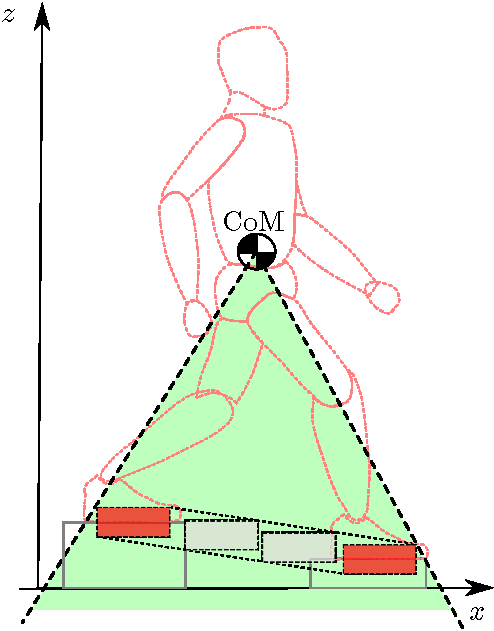
\includegraphics[width=0.45\textwidth]{figures/SYROCO18-double-support3D.pdf}
    \caption{During double support, the box constraint slides from the
        previous to the next support foot \cite{Zamparelli2018SYROCO}.}
    \label{fig:SYROCO18-double-support3D}
\end{figure}

Because of its constant orientation in the prediction, at each time we can
choose the orientation of the axes to align with the orientation of the moving
box (taken as the orientation of the current support foot) and obtain a ZMP
constraint that is decoupled along the 3 axes. We can write it as
\begin{align}
    \label{eq:ZMP-constraints}
    \begin{split}
        \bm{X}_z^{\rm m,k+1} \le \bm{X}_z^{k+1} \le \bm{X}_z^{M,k+1} \\
        \bm{Y}_z^{\rm m,k+1} \le \bm{Y}_z^{k+1} \le \bm{Y}_z^{M,k+1} \\
        \bm{Z}_z^{\rm m,k+1} \le \bm{Z}_z^{k+1} \le \bm{Z}_z^{M,k+1},
    \end{split}
\end{align}
where $\bm{X}_z^{\rm m,k+1}, \bm{X}_z^{\rm M,k+1}, \bm{Y}_z^{\rm m,k+1},
\bm{Y}_z^{\rm M,k+1}, \bm{Z}_z^{\rm m,k+1}, \bm{Z}_z^{\rm M,k+1}$
are the ZMP bounds along the prediction, which can be expressed as
\begin{equation}
    \begin{aligned}
        \bm{X}_z^{\rm m,k+1} &= \bm{X}_{\rm mc}^{k+1} - \bfz \frac{d_x}{2} &
        \bm{X}_z^{\rm M,k+1} &= \bm{X}_{\rm mc}^{k+1} + \bfz \frac{d_x}{2} \\
        \bm{Y}_z^{\rm m,k+1} &= \bm{Y}_{\rm mc}^{k+1} - \bfz \frac{d_y}{2} &
        \bm{Y}_z^{\rm M,k+1} &= \bm{Y}_{\rm mc}^{k+1} + \bfz \frac{d_y}{2} \\
        \bm{Z}_z^{\rm m,k+1} &= \bm{Z}_{\rm mc}^{k+1} - \bfz \frac{d_z}{2} &
        \bm{Z}_z^{\rm M,k+1} &= \bm{Z}_{\rm mc}^{k+1} + \bfz \frac{d_z}{2}.
    \end{aligned}
\label{eq:FAPA:zmp_constraint_displacement}
\end{equation}
The size of the moving box $(d_x, d_y, d_z)^T$ is
determined in such a way to always be contained inside the pyramid $\cal Z$
\cite{Zamparelli2018SYROCO, Cipriano2023RAS}.
The center of the moving box $\bfp_{\rm mc}$ must be expressed in terms of
the subplan $\mathcal{P}^l$. First we define the {\em piecewise-linear sigmoid}
function 
\begin{equation*}
\sigma (t,t_i,t_f)=\frac{1}{t_f-t_i} \left(\rho(t-t_i)-\rho(t-t_f)\right),
%\label{eq:FAPA:sigma}
\end{equation*}
where $\rho(t)=t\delta_{-1}(t)$ is the unit ramp.
$\sigma (t,t_i,t_f)$ is 0 before $t_i$,  1 after $t_f$, and it transitions
linearly in the interval $[t_i,t_f]$. This function is useful to represent
the transition between consecutive footsteps.

The vectors $\bm{X}_{\rm mc}^{k+1}, \bm{Y}_{\rm mc}^{k+1}, \bm{Z}_{\rm mc}^{k+1}$
collecting the positions of the moving constraint along the horizon
can be written as
\begin{equation}
    \begin{aligned}
        \bm{X}_{\rm mc}^{k+1} = \bm{M} \bm{X}_f^l + \bm{m}x_f^l \\
        \bm{Y}_{\rm mc}^{k+1} = \bm{M} \bm{Y}_f^l + \bm{m}y_f^l \\
        \bm{Z}_{\rm mc}^{k+1} = \bm{M} \bm{Z}_f^l + \bm{m}z_f^l
    \end{aligned}
    \label{eq:FAPA:mapping}
\end{equation}
where
\begin{equation*}
    \begin{aligned}
        \bm{X}_{f}^{l} &= (x_{f}^{l} \ x_{f}^{l+1} \ \dots \ x_{f}^{l+F})^T \\
        \bm{Y}_{f}^{l} &= (y_{f}^{l} \ y_{f}^{l+1} \ \dots \ y_{f}^{l+F})^T \\
        \bm{Z}_{f}^{l} &= (z_{f}^{l} \ z_{f}^{l+1} \ \dots \ z_{f}^{l+F})^T
    \end{aligned}
\end{equation*}
collect the footstep positions.
$\bm{M}\in\mathbb{R}^{C\times F}$ is a mapping matrix whose elements
$M_{ij}$ are defined as
\begin{equation}\begin{split}
M_{ij} &= \sigma(t_{k+i}, t_s^{l+j},t_s^{l+j}+T_{\rm ds}^{l+j})\\ &- \sigma(t_{k+i}, t_s^{l+j-1},t_s^{l+j-1}+T_{\rm ds}^{l+j-1}),
\end{split}\end{equation}
and $\bfm\in\mathbb{R}^{C}$ is a vector whose elements $m_i$ are given by
\begin{equation*}
m_{i} = 1 - \sigma(t_{k+i}, t_s^{l},t_s^{l}+T_{\rm ds}^{1}),
\end{equation*}
where $t_s^l$ is the starting time of the $l$-th step and
\begin{equation*}
    t^j_s = t^l_s + \sum^{l+j-1}_{\lambda=l} \left(T_{\rm ds}^\lambda + T_{\rm ss}^\lambda\right).
\end{equation*}

\section{IS-MPC algorithm}
IS-MPC solves, at each time $t_k$, the following QP problem:
\begin{braced}
\begin{equation}
\begin{split}
\min_{\dot{\bm{X}}_\text{z}^k, \dot{\bm{Y}}_\text{z}^k, \dot{\bm{Z}}_\text{z}^k}
&\|\dot{\bm{X}}_z^k\|^2 + \|\dot{\bm{Y}}_z^k\|^2 + \|\dot{\bm{Z}}_z^k\|^2+\beta \|\bm{X}_z^{k+1} - \bfX_{\rm mc}^{k+1}\|^2 \\& + \beta \|\bm{Y}_z^{k+1} - \bfY_{\rm mc}^{k+1}\|^2 + \beta \|\bm{Z}_z^{k+1} - \bfZ_{\rm mc}^{k+1}\|^2 \\
\end{split}
\label{eq:ISMPC-algorithm}
\end{equation}
\hspace{0.25cm} subject to:
\begin{itemize}
    \item stability constraints (\ref{eq:stability-constraint-matrix})
    \item ZMP constraints (\ref{eq:ZMP-constraints})
\end{itemize}
\end{braced}

In the cost function, the first three terms act as regularization while the
remaining attempt to bring the ZMP as close as possible to the center of the
moving box, with a strength modulated by the weight $\beta$.

The first sample $\dot \bfp_z^k = (\dot x_z^k, \dot y_z^k, \dot z_z^k)$ of the
optimal sequence is used to integrate the prediction model and the resulting
CoM position $\bfp_c^{k+1}$ is sent to the kinematic controller together with
a suitable swing foot trajectory that allows to reach the target footstep
position at the proper time.

\section{Feasibility region}

The {\em feasibility region} is the region of the state space in which the
IS-MPC optimization problem \eqref{eq:ISMPC-algorithm} is feasible.

\begin{proposition}
\label{prop:feasibility}
IS-MPC is feasible at time $t_k$ if
\begin{align}
\label{eq:FAPA:mpc-feasibility-constraint}
\bm{s}^T \bm{P}^{-1} (\bm{X}_z^{{\rm m}, k+1} \!-\! \bm{p} x_z^k)  \!&\le\! x_u^k \!+\! b_x^k \!\le\! \bm{s}^T \bm{P}^{-1} (\bm{X}_z^{{\rm M}, k+1} \!-\! \bm{p} x_z^k),
\nonumber\\
\bm{s}^T \bm{P}^{-1} (\bm{Y}_z^{{\rm m}, k+1} \!-\! \bm{p} y_z^k)  \!&\le\! y_u^k \!+\! b_y^k \!\le\! \bm{s}^T \bm{P}^{-1} (\bm{Y}_z^{{\rm M}, k+1} \!-\! \bm{p} y_z^k),
\nonumber\\
\bm{s}^T \bm{P}^{-1} (\bm{Z}_z^{{\rm m}, k+1} \!-\! \bm{p} z_z^k)  \!&\le\! z_u^k \!+\! b_z^k \!\le\! \bm{s}^T \bm{P}^{-1} (\bm{Z}_z^{{\rm M}, k+1} \!-\! \bm{p} z_z^k).
\end{align}
\end{proposition}
{\em Proof}.
We focus the proof on the inequalities for the $x$ component, as the logic, for
the other components is identical. The bounds of the feasibility region along
$x$ are given by
\begin{align*}
x_u^{k,b1} &= \bm{s}^T \bm{P}^{-1} (\bm{X}_z^{{\rm m}, k+1} - \bm{p} x_z^k) - b_x^k, \\
x_u^{k,b2} &= \bm{s}^T \bm{P}^{-1} (\bm{X}_z^{{\rm M}, k+1} - \bm{p} x_z^k) - b_x^k.
\end{align*}
Then, if $x_u^k$ is inside the feasibility region, it is possible to express
it as a convex combination of the two bounds, i.e.,
\begin{equation}\label{eq:FAPA:xu_convex}
x_u^k = \alpha x_u^{k,b1} + (1-\alpha)x_u^{k,b2}, \alpha \in [0, 1].
\end{equation}

Consider the following ZMP velocity trajectory:
\begin{equation}\label{eq:FAPA:candidate_trajectory}
\dot{\bm{X}}_z^k = \alpha \bm{P}^{-1}(\bm{X}_z^{{\rm m}, k+1} - \bm{p} x_z^k) + (1-\alpha)\bm{P}^{-1}(\bm{X}_z^{{\rm M}, k+1} - \bm{p} x_z^k).
\end{equation}
We will show that this particular trajectory satisfies both the stability
constraint and the ZMP constraints. As for the stability constraint, multiply
both sides of (\ref{eq:FAPA:candidate_trajectory}) by $\bm{s}^T$
% \begin{equation}
% \bm{s}^T\bm{\dot X}_z^k = \bm{s}^T(\alpha \bm{Z}^{-1}(\bm{X}_z^{{\rm m}, k+1} - \bm{z} x_z^k) + (1-\alpha)\bm{Z}^{-1}(\bm{X}_z^{{\rm M}, k+1} - \bm{z} x_z^k)),
% \end{equation}
and plug in the definitions of $x_u^{k,b1}$ and $x_u^{k,b2}$ to obtain
\begin{equation*}
\bm{s}^T\dot{\bm X}_z^k = (\alpha (x_u^{k,b1} + b^k_x)) + (1-\alpha)(x_u^{k,b2} + b^k_x)).
\end{equation*}
Using (\ref{eq:FAPA:xu_convex}), this is equivalent to the stability
constraint (\ref{eq:stability-constraint-matrix}).

To prove satisfaction of the ZMP constraint. Left-multiplying
\eqref{eq:ZMP-positions-x-matrix} by $\bm{Z}$, the chosen ZMP velocity
trajectory can be rewritten as
\begin{equation*}
\bm{X}_z^k - \bm{p} x_z^k = \alpha (\bm{X}_z^{{\rm m}, k+1} - \bm{p} x_z^k) + (1-\alpha)(\bm{X}_z^{{\rm M}, k+1} - \bm{p} x_z^k),
\end{equation*}
which simplifies to
$\bm{X}_z^k = \alpha \bm{X}_z^{{\rm m}, k+1} + (1-\alpha)\bm{X}_z^{{\rm M}, k+1}$,
and therefore the ZMP constraint (\ref{eq:ZMP-constraints}) is satisfied.
\hfill\bull

Note that, because $\bm{P}$ is a lower-triangular matrix filled with $\delta$,
its inverse is simply
\begin{equation*}
    \bm{P}^{-1}
    =
    \begin{bmatrix}
         1/\delta &         0 &        0 &  \dots &         0 &        0 \\
        -1/\delta &  1/\delta &        0 &  \dots &         0 &        0 \\
                0 & -1/\delta & 1/\delta &  \dots &         0 &        0 \\
           \vdots &    \vdots &   \vdots & \vdots &    \vdots &   \vdots \\
                0 &         0 &        0 &  \dots &  1/\delta &        0 \\
                0 &         0 &        0 &  \dots & -1/\delta & 1/\delta
    \end{bmatrix}.
\end{equation*}
